
%%%%%%%%%%%%%%%%%%%%%%%%%%%%%%%%%%%%%%%%%%%%%%%%%%%
%% Capítulo 1: El Concepto de Fractal
%%%%%%%%%%%%%%%%%%%%%%%%%%%%%%%%%%%%%%%%%%%%%%%%%%%


Las primeras preguntas que se pueden plantear son ¿qué es un fractal? ¿Qué tienen de especial estas figuras? ¿Qué las diferencia de un objeto no fractal? ¿Por qué es necesaria una geometría fractal? Trataremos de responder a cada una de estas preguntas a lo largo de este capítulo, comenzando por la primera de ellas. En realidad, hay distintas definiciones de \textit{fractal}, pero todas utilizan dos conceptos como base: la \textbf{autosimilaridad} y la \textbf{dimensión}. La primera de ellas es más cercana para nosotros de lo que en un principio podemos pensar, fijémonos en los ejemplos de la imagen \ref{fig:objetos}. 

\begin{figure}[ht]
\begin{tabular}{cc}
  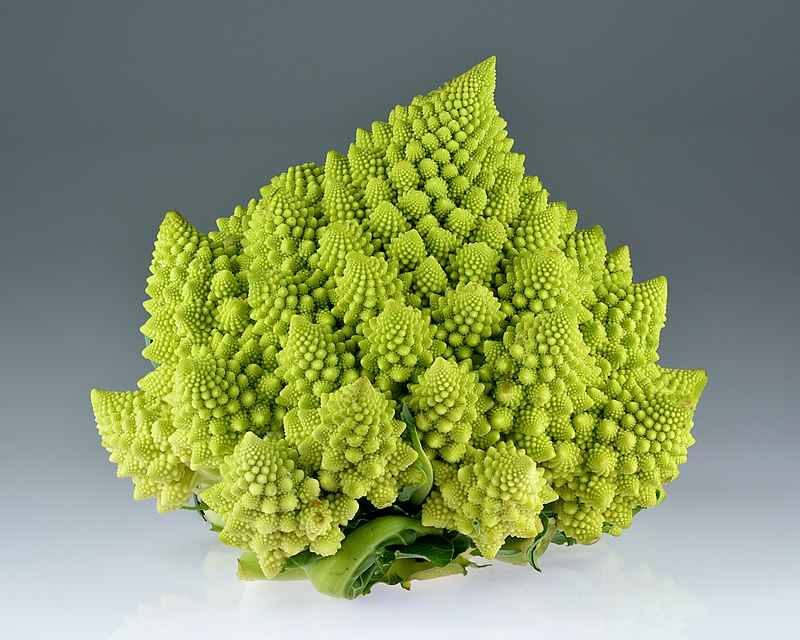
\includegraphics[scale=0.225]{./img/romanescu.jpg} &   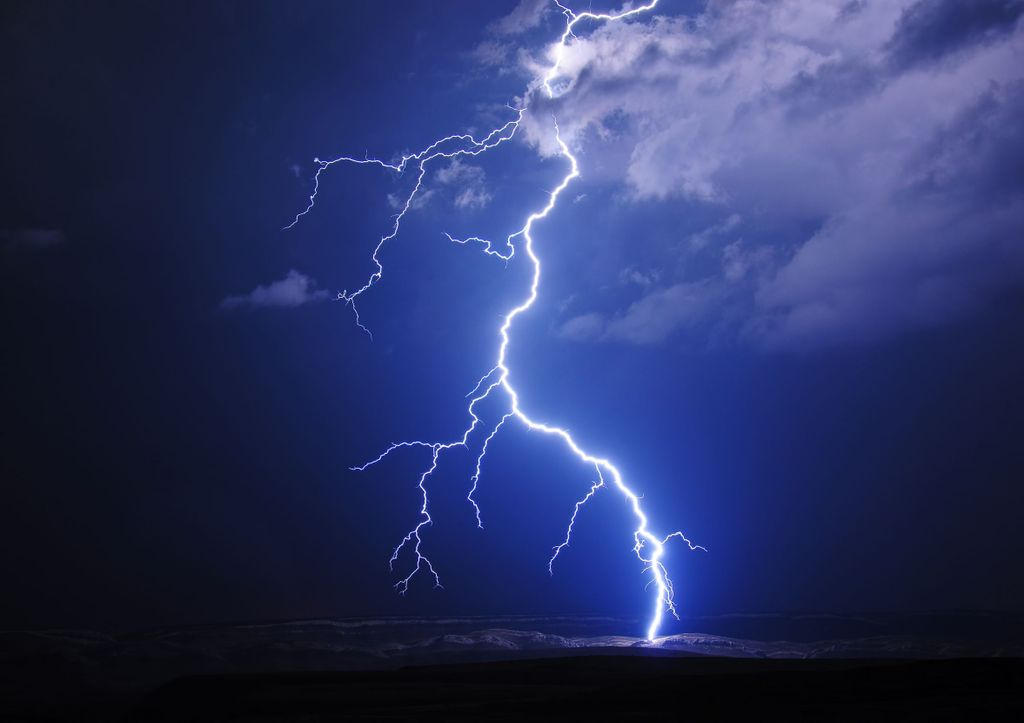
\includegraphics[scale=0.2]{./img/rayo.jpg} \\
(a) Romanescu & (b) Rayo \\[6pt]
\end{tabular}
\caption{Objetos de la naturaleza con estructura fractal}
\label{fig:objetos}
\end{figure}

Observemos que el romanescu, que es un tipo de coliflor, pareciera que está formado de pequeños trozos que recuerdan el objeto original, mientras que estos pequeños trozos a su vez también están formados de pequeños trozos similares al objeto inicial, y así sucesivamente. Por su parte, el rayo se compone de un destello principal del que salen ramificaciones de las que a su vez se originan otras divisiones, formando pequeños rayos semejantes al rayo primitivo.

Esta idea de objetos prácticamente iguales al original salvo cambios de escala es la subyacente al concepto de autosimilaridad.

\begin{definicion}[Autosimilaridad] Una figura o subconjunto $A$ de $\R^n$ es \textbf{autosimilar} si está compuesto por copias de sí mismo reducidas mediante un factor de escala y desplazadas por un movimiento rígido. Es decir,
$$
A = \bigcup_{i=1}^n f_i\circ h_i(A),
$$
donde cada $h_i, i=1,\dots,n$ es una homotecia de razón menor que 1 y $f_i, i=1,\dots,n$ es un movimiento rígido. 
\end{definicion}

En futuras ocasiones se utilizarán indistintamente los términos de <<reducción por un factor de escala>> e <<imagen vía una homotecia>>, evidenciando el movimiento rígido y queriendo en ambos casos referirnos a este concepto.

Para afianzar y formalizar conceptos y con el objetivo de introducir una definición de la dimensión, estudiaremos algunos ejemplos clásicos de objetos fractales.

\section{Ejemplos clásicos}
\label{section:ejemplos}

En adelante, y salvo que se indique lo contrario, cuando hablemos en términos topológicos de $\R^n$ o subconjuntos suyos nos estaremos refiriendo al espacio topológico $\R^n$ dotado de la topología usual o la topología inducida por la usual en el caso de subconjuntos de $\R^n$.

\subsection{El conjunto de Cantor}
\label{subsection:Cantor}

Creado por el célebre matemático \textit{George Cantor}, este fractal se construye a partir de un segmento de línea recta aplicando el siguiente proceso iterativo:

\begin{enumerate}
\item Partimos del segmento de recta compuesto por el intervalo cerrado $[0,1]$, aunque realmente es indiferente qué intervalo se escoja, pues el resultado final será el mismo salvo homotecia. Dividimos dicho segmento en tres segmentos iguales y extraemos el intervalo central, manteniendo los extremos. Es decir, extraemos el intervalo abierto $\left(\frac 1 3, \frac 2 3\right)$ y mantenemos el segmento $\left[0,\frac 1 3\right]$ y el $\left[\frac 2 3, 1\right]$.. Nótese que obtenemos $2=2^1$ segmentos, cada uno a escala $\frac 1 3=\left(\frac 1 3\right)^1$ del original.

\item Aplicamos el mismo proceso a los segmentos $\left[0,\frac 1 3\right]$ y $\left[\frac 2 3, 1\right]$. Esto es, se dividen ambos en tres partes iguales y se extrae el intervalo abierto central de cada uno de ellos, manteniendo los extremos. En este caso obtendríamos $4=2^2$ segmentos iguales, cada uno de ellos a escala $\frac 1 3$ de los dos obtenidos en el primer paso y a escala $\frac 1 9=\left(\frac 1 3\right)^2$ del original.

\item Repetimos este proceso de manera indefinida, de manera que en el $n$-ésimo paso se obtendrían $2^n$ segmentos de recta a escala $\left(\frac 1 3\right)^n$. Denotemos como $C_n$ al conjunto unión de los $2^n$ segmentos de recta que se generan en el paso $n$ del proceso.
\end{enumerate} 

Los puntos del intervalo inicial $[0,1]$ que restan tras las infinitas iteraciones son los que conforman el \textit{conjunto de Cantor}, que denotamos con $\mathbf{C}$, de forma que $\mathbf{C}=\bigcap_{n\in\N}C_n$.

\begin{figure} [ht]
\centering
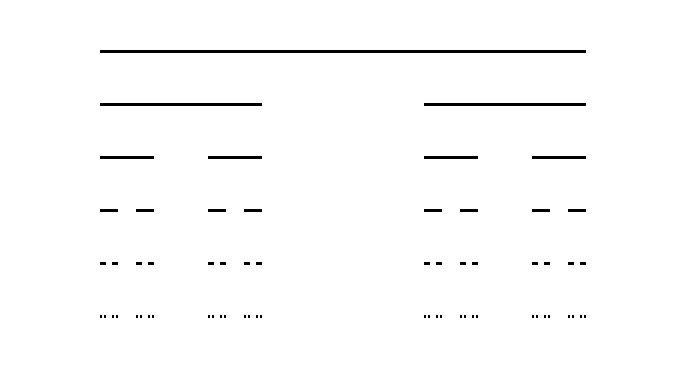
\includegraphics[scale = 0.4]{img/cantor.png}
\caption{Iteraciones del proceso de generación del conjunto de Cantor}
 \label{fig:Cantor}
\end{figure}

El conjunto de Cantor es además un conjunto compacto, pues cada $C_n$ es una unión finita de intervalos cerrados y acotados de $\R$, y por tanto compactos, como sabemos gracias al \textit{teorema de Heine-Borel}. Sabiendo que la intersección arbitraria de conjuntos cerrados es cerrada, y que cada $C_n$ está acotado, tenemos pues que $\mathbf{C}$ es un conjunto compacto.

Observemos ahora que en la primera iteración eliminamos $1$ segmento de longitud $\frac 1 3$, en la segunda iteración se eliminan $2$ segmentos de longitud $\left(\frac{1}{3}\right)^2$ y en la $n$-ésima iteración extraemos $2^{n-1}$ segmentos de longitud $\left(\frac{1}{3}\right)^n$. Si sumamos las longitudes de todos los segmentos que son eliminados en cada paso se obtiene:
$$
\sum_{n=1}^\infty 2^{n-1}\left(\frac 1 3\right)^n  = \frac 1 3  \sum_{n=0}^\infty 2^n\left(\frac 1 3\right)^n =  \frac 1 3  \sum_{n=0}^\infty \left(\frac 2 3\right)^n = \frac{1}{3} \left(\frac{1}{1-\frac{2}{3}}\right) = 1,
$$
donde hemos usado que la suma de una serie geométrica de razón $|q|<1$ es $\sum_{n=0}^\infty q^n = \frac{1}{1-q}$.

Esto nos lleva a concluir que la longitud eliminada es igual a la longitud original, es decir, la longitud de $\mathbf C$ es nula y aún así tenemos puntos, por ejemplo los extremos de los intervalos que se van generando. Es decir, los puntos de $\mathbf{C}$ no están agrupados, sino que forman una especie de \textit{polvareda}.

\subsection{El triángulo de Sierpinski}
\label{subsection:triangulo-Sierpinski} 

Esta figura, original del polaco \textit{Waclaw Sierpinski}, es creada de una manera que evoca al conjunto de Cantor, pero en dos dimensiones. Veamos detalladamente el proceso (ver imagen \ref{fig:triangulo-Sierpinski}):

\begin{enumerate}
\item Se parte de un triángulo equilátero de lado 1 (de nuevo la longitud inicial es irrelevante). Uniendo los puntos medios de cada lado obtenemos una partición del triángulo inicial en 4 triángulos equiláteros, del cual extraemos el interior del triángulo central. Tenemos por tanto $3=3^1$ triángulos a escala $\frac 1 2 = \left(\frac 1 2\right)^1$ del original.

\item En cada uno de estos tres triángulos equiláteros se repite la operación anterior, obteniendo por tanto $9=3^2$ triángulos, cada uno a escala $\frac 1 4 = \left(\frac 1 2\right)^2$ del original.

\item Repetimos este proceso indefinidamente, de forma que en el paso $n$-ésimo se tienen $3^n$ triángulos, cada uno de ellos a escala $\left(\frac 1 2\right)^n$ del original.
\end{enumerate}

La figura a la que converge este proceso infinito se conoce como triángulo \textbf{S} de Sierpinski.

\begin{figure} [ht]
\centering
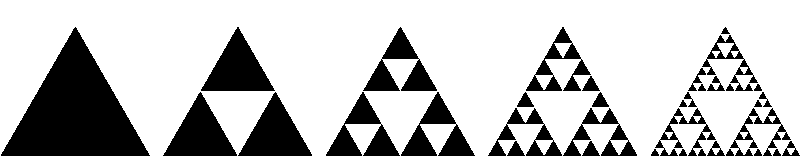
\includegraphics[scale = 0.6]{img/Sierpinski-triangle.png}
\caption{Generación del triángulo de Sierpinski}
 \label{fig:triangulo-Sierpinski}
\end{figure}

Si llamamos $A$ al área del triángulo inicial, sabemos que en la primera iteración eliminamos un área de $\frac 1 4 A$, en el segundo eliminamos $3 \left(\frac 1 4\right)^2 A$ y en el $n$-ésimo $3^{n-1}\left(\frac 1 4\right)^n A$, de forma que si sumamos todo el área que eliminamos en cada paso obtenemos:
$$
A \sum_{n=1}^\infty 3^{n-1}\left(\frac 1 4\right)^n  = \frac A 4  \sum_{n=0}^\infty 3^n\left(\frac 1 4\right)^n =  \frac A 4  \sum_{n=0}^\infty \left(\frac 3 4\right)^n = \frac{A}{4} \left(\frac{1}{1-\frac{3}{4}}\right) = A,
$$

En este caso ocurre algo parecido a lo que vimos que sucedía con el conjunto de Cantor en la sección \ref{subsection:Cantor}. El área eliminada es igual al área total, es decir, su área es 0 y seguimos tenemos puntos (por ejemplo los vértices de los triángulos originados en cada iteración). Es decir, los puntos que forman \textbf{S} no están agrupados formando un área.

\subsection{La alfombra de Sierpinski y la esponja de Menger}
\label{subsection:alfombra-esponja}

El propio Sierpinski se dio cuenta que con el mismo patrón utilizado para generar \textbf{S} se pueden obtener otras formas. Por ejemplo, pensemos que en lugar de comenzar con un triángulo equilátero partimos de un cuadrado, lo subdividimos en 9 cuadrados de lado $\frac 1 3$ y extraemos el cuadrado central. Repitiendo este proceso indefinidamente con cada uno de los cuadrados que se generan finalmente se obtiene la llamada alfombra de Sierpinski (ver imagen \ref{fig:alfombra-Sierpinski}).

\begin{figure} [ht]
\centering
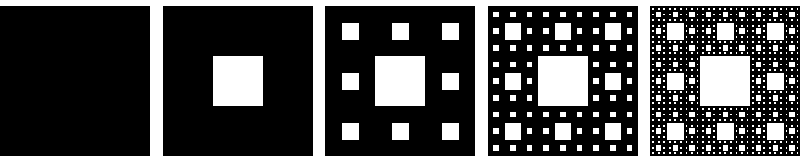
\includegraphics[scale = 0.6]{img/Sierpinski-carpet.png}
\caption{Generación de la alfombra de Sierpinski}
 \label{fig:alfombra-Sierpinski}
\end{figure}

Este proceso también se puede modelar en 3D, obteniendo así la conocida como esponja de Menger o cubo de Magritte, que es una generalización en tres dimensiones de la alfombra de Sierpinski, la cual podemos ver en la imagen \ref{fig:esponja-menger}.

\begin{figure} [ht]
\centering
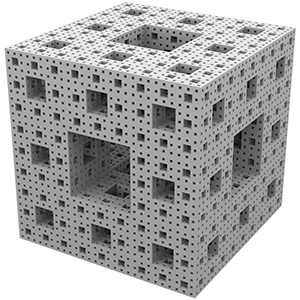
\includegraphics[scale = 0.6]{img/esponja_menger.png}
\caption{Esponja de Menger}
 \label{fig:esponja-menger}
\end{figure}

\subsection{La curva de Koch}
\label{subsection:curva-Koch}

Esta figura fractal, creada por el sueco \textit{N. F. Helge von Koch} sigue un proceso de construcción iterativo al igual que el conjunto de Cantor, pero en lugar de eliminar segmentos, se añaden de la siguiente manera (ver imagen \ref{fig:curva-Koch}):

\begin{enumerate}
\item Partiendo de un segmento de recta de longitud $1$ (al igual que en el conjunto de Cantor, la longitud del segmento inicial es irrelevante, pues la figura final es la misma salvo homotecia), se divide en tres partes iguales de longitud $\frac 1 3$ y la parte central se sustituye por un triángulo equilátero al que se le elimina la base. Esto da lugar a $4=4^1$ segmentos de recta de longitud $\frac 1 3=\left(\frac 1 3\right)^1$.

\item Repetimos este proceso en cada uno de los segmentos de recta obtenidos, colocando el triángulo siempre por encima de la recta, obteniendo así $16=4^2$ segmentos de recta de longitud $\frac 1 9=\left(\frac 1 3\right)^2$.

\item Aplicamos este proceso indefinidamente, obteniendo en el paso $n$-ésimo $4^n$ segmentos de longitud $\left(\frac 1 3\right)^n$. 
\end{enumerate}

El resultado final del proceso es lo que llamamos la \textit{curva de Koch}, que denotamos como \textbf{K}.

\begin{figure} [ht]
\centering
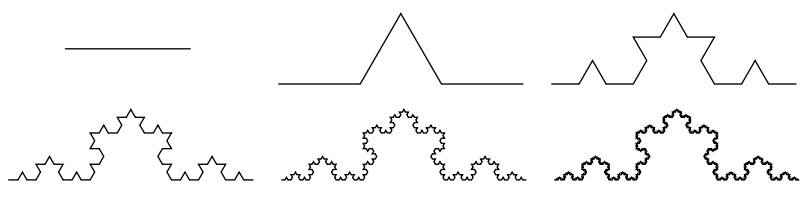
\includegraphics[scale = 0.5]{img/curva-Koch.png}
\caption{Iteraciones del proceso de generación de la curva de Koch}
 \label{fig:curva-Koch}
\end{figure}

\subsection{El copo de nieve de Koch}
\label{subsection:copo-Koch}

A partir de la curva de Koch podemos generar un objeto matemático muy particular: el copo de nieve de Koch. Para crearlo, basta aplicar el proceso iterativo descrito para generar la curva de Koch a cada uno de los segmentos que componen un triángulo equilátero, de forma que los triángulos que se generan apunten hacia el exterior.


\begin{figure} [ht]
\centering
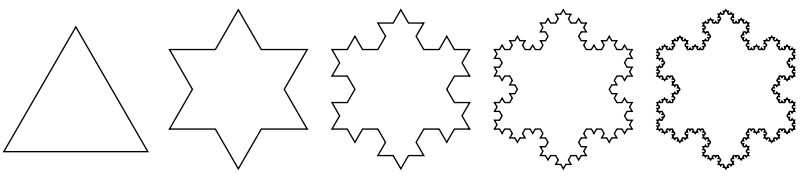
\includegraphics[scale = 0.6]{img/copo-Koch.png}
\caption{Generación del copo de nieve de Koch}
\label{fig:copo-Koch}
\end{figure}

Esta curva posee la particularidad de tener longitud infinita y a su vez encerrar un área finita. Realmente el copo de Koch no es exactamente un fractal, pues no es totalmente autosimilar, aunque se compone de tres partes idénticas las cuales sí son autosimilares, como podemos ver en la imagen \ref{fig:copo-Koch-colores}.

\begin{figure} [ht]
\centering
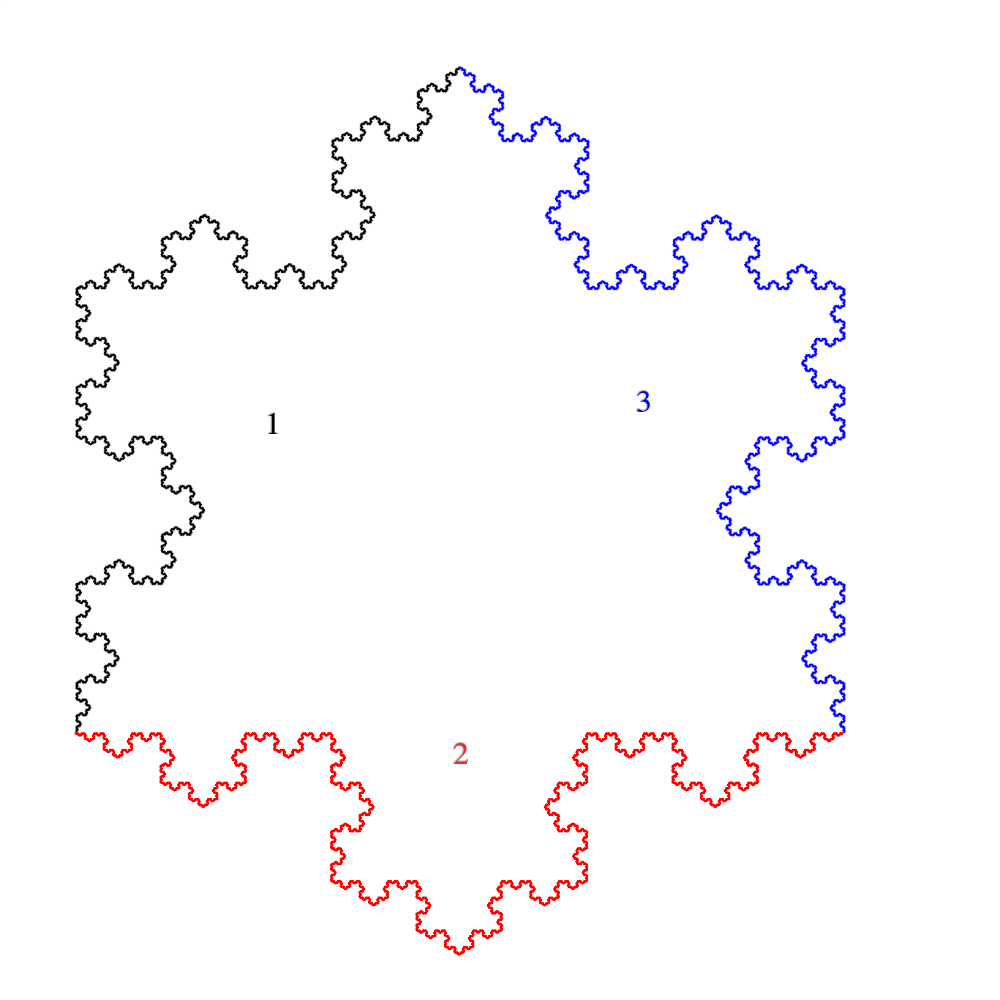
\includegraphics[scale = 0.2]{img/copo-Koch-colores.png}
\caption{Curvas de Koch que componen el copo de Koch}
\label{fig:copo-Koch-colores}
\end{figure}


\section{Conceptos de dimensión fractal}
\label{section:dimension}

Al iniciar este capítulo mencionamos que las distintas definiciones de fractal utilizaban los conceptos de autosimilaridad y dimensión. Con los distintos ejemplos hemos entendido el primero de ellos, por lo que es momento de abordar el concepto de dimensión. 

El concepto de dimensión más clara que tenemos es el de dimensión algebraica, esto es, la dimensión de un espacio vectorial. Sabemos que un espacio vectorial $V$ se dice que tiene $\dim(V)=n$, con $n\in\N$ si, y solo si existe una base de $V$ constituida por $n$ vectores, de forma que cualquier elemento de $V$ puede ser expresado como una combinación lineal de los $n$ vectores de la base. Otra manera de ver esto es que para construir los vectores de $V$ tenemos hasta $n$ parámetros de libertad, esto es, $v=a_1 v_1 +\cdots a_n v_n \ \ \forall v\in V$, donde $\{v_1,\dots,v_n\}$ es una base de $V$ y $a_1,\dots,a_n\in K$ siendo $K$ el cuerpo sobre el que está construido el espacio vectorial.

En el caso de subconjuntos de $\R^n$ como puede ser una curva parametrizada, si seguimos la analogía del número de parámetros que define un punto en este caso de una curva, podemos decir que su dimensión es $1$, ya que un punto de una curva parametrizada puede expresarse en función de un único parámetro. La variación de este parámetro nos daría otro punto de la curva, por lo que podemos decir que un punto puede moverse por la curva con un grado de libertad (ver imagen \ref{fig:curva-superficie} (a)). Por su lado, una superficie regular de $\R^3$ puede localmente ser expresada como la imagen de una parametrización que depende de dos variables y la variación de estas mediante dicha parametrización resulta en otro punto de la superficie, pudiendo expresar esto como que un punto de una superficie regular tiene dos grados de libertad, lo que intuitivamente permite afirmar que una superficie regular tiene dimensión $2$ (ver imagen \ref{fig:curva-superficie} (b)).

\begin{figure}[ht]
\centering
\begin{tabular}{cc}
  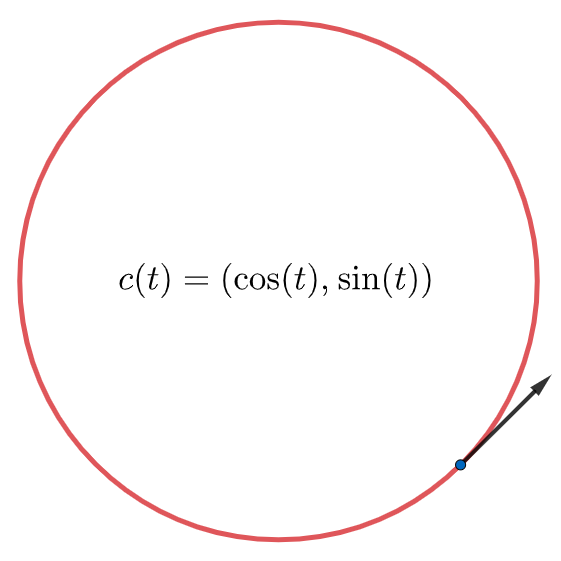
\includegraphics[scale=0.3]{./img/circunferencia.png} &   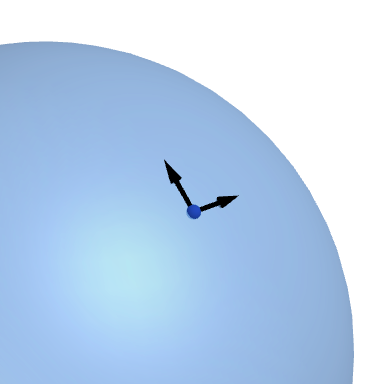
\includegraphics[scale=0.5]{./img/esfera.png} \\
(a) En una curva de $\R^2$ & (b) En una superficie de $\R^3$ \\[4pt]
\end{tabular}
\caption{Posible movimiento de un punto en posibles objetos de $\R^n$}
\label{fig:curva-superficie}
\end{figure}

Un posible enfoque para definir la dimensión puede ser el recién presentado, el cual nos sugiere pensar en el número de parámetros que definen la libertad de movimiento de un punto. Sin embargo, pensemos ahora en el triángulo de Sierpinski y en su dimensión. Comprobamos en la sección \ref{subsection:triangulo-Sierpinski} que su área 2-dimensional es nula, pero en el objeto final pareciera que un punto se pudiera mover en varias direcciones. No se puede afirmar que \textbf{S} tenga dimensión 1 por la movilidad, pero tampoco dimensión 2 porque tiene área 0, pero sería un valor situado entre estos dos enteros.

\subsection{Dimension fractal autosimilar}
\label{subsection:dim-frac-autosimilar}

Pensemos ahora en un segmento de recta, un cuadrado y un cubo, que son objetos indudablemente de 1, 2 y 3 dimensiones respectivamente. Ahora dividamos los lados de cada objeto en 2 tal y como indica la imagen \ref{fig:divisiones}. Entonces en el segmento aparecen $N(2):=2=2^1$ segmentos que son imagen de una homotecia de razón $r=\frac 1 2$ del original, en el cuadrado se obtienen $N(2):=4=2^2$ cuadrados, cada uno imagen de una homotecia de razón $\frac 1 2$ del cuadrado inicial y en el cubo $N(2):=8=2^3$ cubos, de nuevo cada uno de ellos imagen de una homotecia de razón $\frac 1 2$ del cubo original.

\begin{figure}[ht]
\begin{tabular}{ccc}
  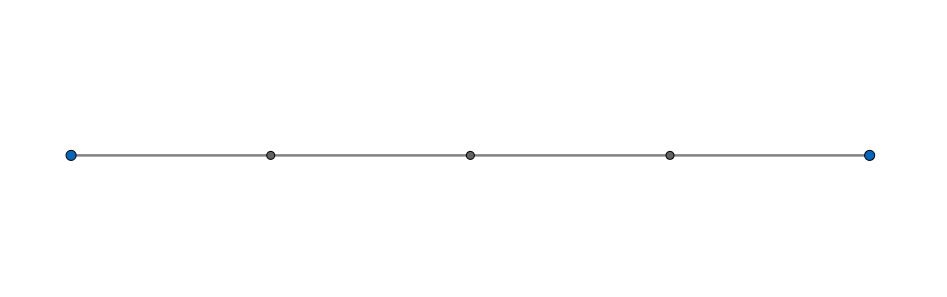
\includegraphics[scale=0.15]{./img/linea-dividida.png} &   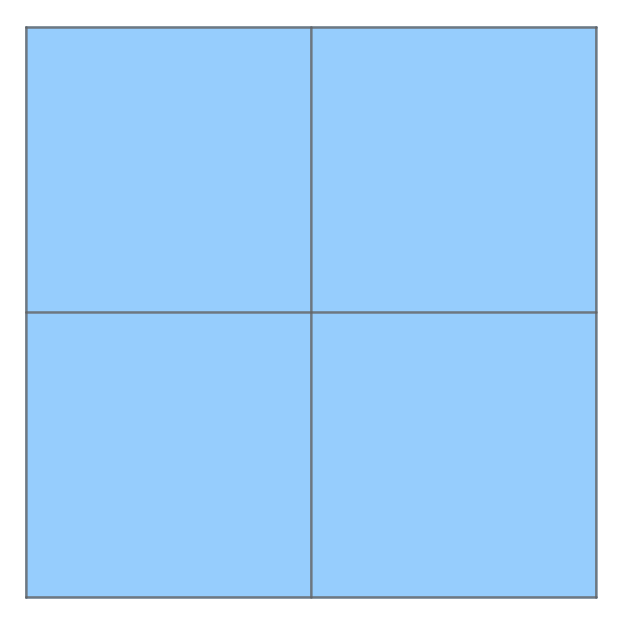
\includegraphics[scale=0.15]{./img/cuadrado-dividido.png} & 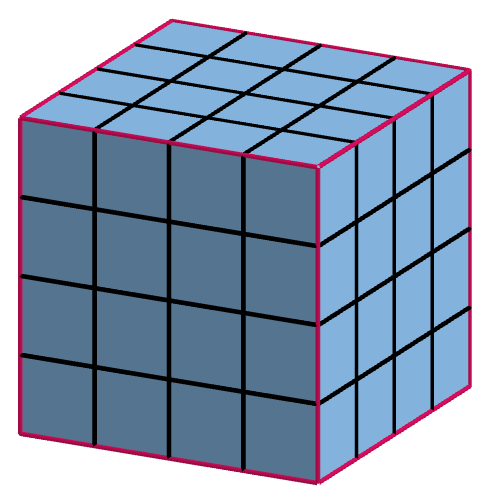
\includegraphics[scale=0.2]{./img/cubo-dividido.png}\\
(a) Segmento dividido en 2 & (b) Cuadrado dividido en 4 & (c) Cubo dividido en 8 \\[4pt]
\end{tabular}
\caption{Segmento, cuadrado y cubo divididos en objetos a razón $\frac 1 2$}
\label{fig:divisiones}
\end{figure}

Si en lugar de 2 tomamos cualquier número natural $k\geq 1$, la razón de la homotecia sería $r=\frac 1 k$ y en ese caso se obtendrían $N(k)=k^1$ segmentos de recta, $N(k)=k^2$ cuadrados y $N(k)=k^3$ cubos, en todos los casos a escala $r=\frac 1 k$ de los objetos originales. Estas igualdades se pueden reescribir como:

\begin{equation}\label{eq:relaciones-dimension}
\frac{N(k)}{k^1}=1 \hspace{2cm} \frac{N(k)}{k^2}=1 \hspace{2cm} \frac{N(k)}{k^3}=1
\end{equation}

En este sentido, vemos que la dimensión de cada objeto es el \textit{exponente} al que habría que elevar la razón de la homotecia $k$ para obtener la relación (\ref{eq:relaciones-dimension}). Para abreviar en el lenguaje introducimos la siguiente definición.

\begin{definicion}[Congruencia]
Dos subconjuntos $A,B$ de $\R^n$ son \textbf{congruentes} si existe un movimiento rígido $f$ tal que $B = f(A)$.
\end{definicion}

De manera análoga al segmento, el cuadrado y el cubo podemos tomar cualquier figura o subconjunto $X\subseteq \R^n$ que pueda ser subdividido en un número finito $N(k)$ de subconjuntos congruentes entre sí y cada uno de ellos imagen por una homotecia de razón $r=\frac 1 k$ de $X$. Esto es, en lenguaje formal, un conjunto autosimilar.

\begin{definicion}[Dimensión autosimilar]
Dado un subconjunto $X$ de $\R^n$ que se puede dividir en $N(k)$ subconjuntos congruentes entre sí y cada uno de ellos imagen por una homotecia de razón $r=\frac 1 k$ de $X$, definimos su \textbf{dimensión autosimilar} como el único valor de $d$ que satisface la identidad $\frac{N(k)}{k^d}=1$, es decir: 
$$
d=\frac{\log N(k)}{\log(k)}
$$
\end{definicion}

También se puede ver definida como \textit{dimensión de homotecia}. Sin embargo, antes de utilizar este concepto debemos comprobar que la definición es coherente con cualquier partición y cualquier factor de escala. Es decir, que independientemente de la división del objeto que se tome la dimensión va a ser la misma.

\begin{proposicion}
En un subconjunto $X$ de $\R^n$ autosimilar el valor de la dimension fractal autosimilar es el mismo independientemente de la partición que se le aplique.
\end{proposicion}
\begin{proof}
TODO
\end{proof}

\begin{wrapfigure}{l}{0cm}
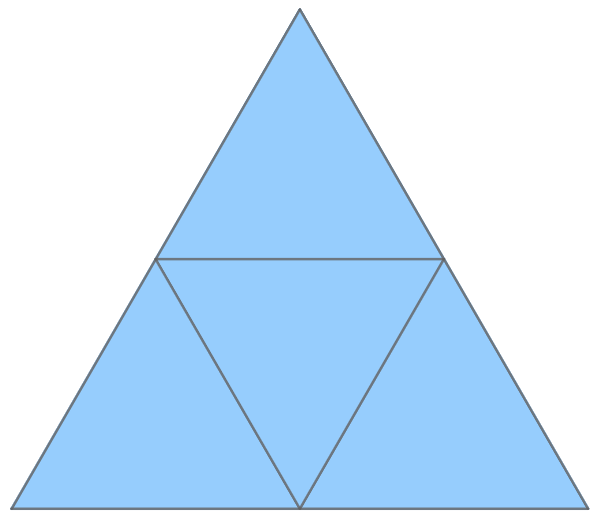
\includegraphics[scale=0.14, trim={0cm 0.35cm 0cm 0.5cm}, clip]{./img/triangulo-dividido.png}
\end{wrapfigure}

Un ejemplo distinto pero clarificador podría ser el de un triángulo equilátero, el cual podemos dividir en 4 copias congruentes entre sí, cada una a escala $r=\frac 1 2$ del triángulo original, de forma que tendríamos $k=2$ y $N(2)=4$. 

Con estos valores, tenemos que $N(k)=4=k^d=2^d$, por lo que necesariamente $d=2$ y por tanto un triángulo equilátero es un objeto 2-dimensional, lo cual tampoco nos sorprende.

\begin{observacion}
La dimensión $d$ ya no tiene por qué ser necesariamente un número entero. A esta posibilidad de tener dimensiones no enteras es a lo que llamamos \textbf{dimensión fractal autosimilar}, y lo denotamos con $\dim_A$.
\end{observacion}

Retomando ahora el triángulo de Sierpinski, sabemos que este está compuesto por 3 copias de sí mismo a escala $\frac 1 2$ (véase sección \ref{subsection:triangulo-Sierpinski}), por lo que entonces su dimensión fractal autosimilar es $\dim_A(\mathbf{S})=\frac{\log 3}{\log 2} \approx 1.58496$. Efectivamente y tal y como discutimos en el inicio de esta sección, es un valor situado entre 1 y 2.

En cuanto al conjunto de Cantor, este está formado por 2 copias de sí mismo a escala $\frac 1 3$ (sección \ref{subsection:Cantor}), por lo que su dimensión fractal autosimilar sería $\dim_A(\mathbf{C})=\frac{\log 2}{\log 3} \approx 0.63093$, que es un valor situado entre 0 y 1.

Por su parte, la curva de Koch se compone de 4 copias de sí misma, cada una a escala $\frac 1 3$ de la curva original (sección \ref{subsection:curva-Koch}). Por tanto, su dimensión fractal autosimilar es $\dim_A(\mathbf{K})=\frac{\log 4}{\log 3} \approx 1.26186$.

\subsection{Dimensión por cajas}
\label{subsection:dim-cajas}

El concepto de dimensión fractal autosimilar tiene el defecto de que está limitado únicamente a objetos totalmente autosimilares, pero la mayoría de objetos no cumple esta propiedad. Para solucionar este problema, introduciremos un nuevo concepto de dimensión. Previamente definimos un término necesario en las futuras definiciones.

\begin{definicion}
Dado un subconjunto $U$ de $\R^n$, definimos su \textbf{diámetro} como:
$$
\diam(U)=\sup \left\lbrace d(x,y): x,y\in U\right\rbrace .
$$
\end{definicion}

Dado un conjunto $A\subset \R^n$ no vacío y acotado, sea $N_\delta(A)$ el mínimo número de conjuntos de diámetro a lo sumo $\delta$ necesario para recubrir $A$. La \textit{dimensión por cajas superior} y la \textit{dimensión por cajas inferior} se definen, respectivamente como

$$
\diminf(A) := \liminf_{\delta\rightarrow 0}\frac{\log(N_\delta(A))}{\log(1/\delta)},
$$
$$
\dimsup(A) := \limsup_{\delta\rightarrow 0}\frac{\log(N_\delta(A))}{\log(1/\delta)}.\footnote{Nótese la analogía con la notación de los límites superior e inferior como $\varliminf$ y $\varlimsup$. }
$$


En caso de coincidir, se denomina \textit{dimensión por cajas} de $A$ al valor 
\begin{equation}
  \label{eq:dim-cajas}
  \dim_{B}(A) := \lim_{\delta\rightarrow 0}\frac{\log(N_\delta(A))}{\log(1/\delta)}.
\end{equation}

También es conocida en literatura como \textit{dimensión por conteo de cajas} o \textit{dimensión de Minkowski-Bouligand}.

Hay varias definiciones equivalentes, generalmente más sencillas de utilizar. Por ejemplo, si tomamos en $\R^n$ una cuadrícula de lado $\delta$, \textit{i.e.}, de la forma
$$
[m_1 \delta, (m_1+1)\delta]\times\cdots\times[m_n \delta, (m_n+1)\delta]
$$
donde $m_1,\dots,m_n$ son enteros, tendríamos $\R^n$ dividido en `cajas', de diámetro $\delta\sqrt{n}$ y contando el número de cajas que recubren a $A$, obtenemos el mismo resultado, puede comprobarse en \cite[sección 3.1]{alma991007022459704990}.

\begin{figure}[ht]
\begin{tabular}{cc}
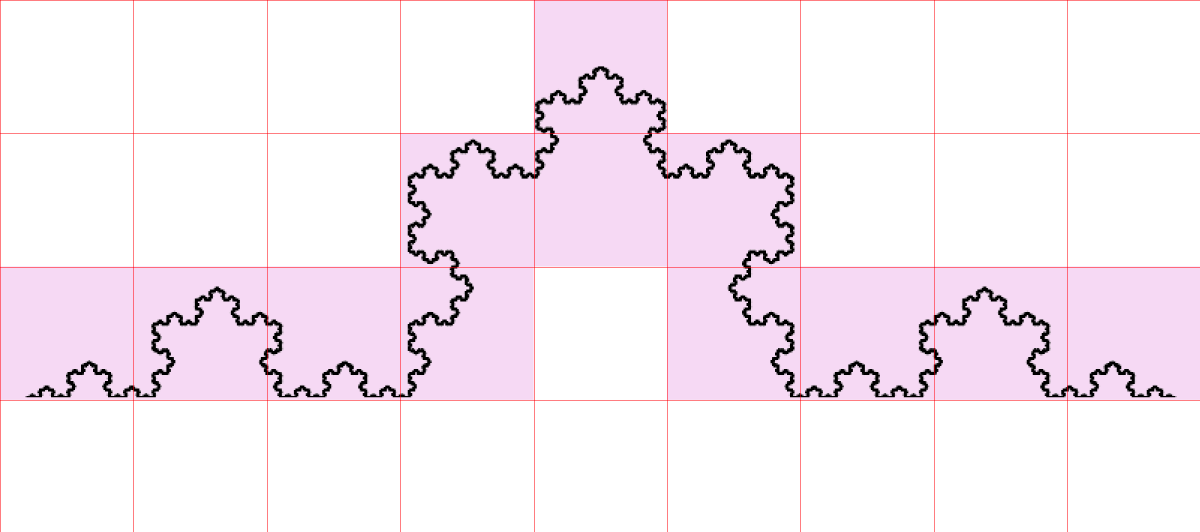
\includegraphics[scale=0.17]{./img/cajas-grandes.png} &   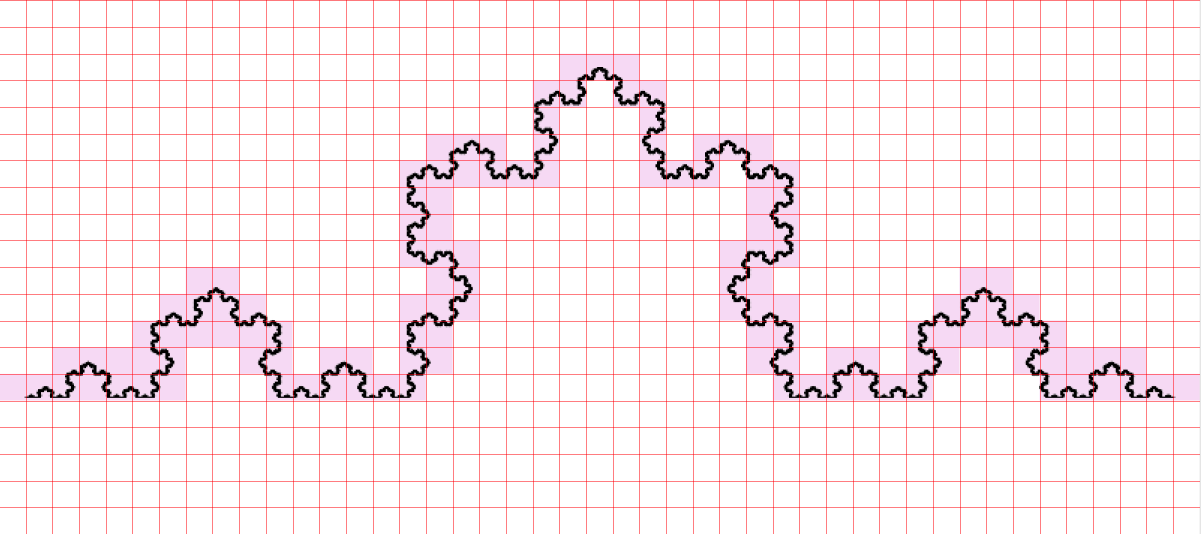
\includegraphics[scale=0.17]{./img/cajas-peques.png} \\
\end{tabular}
\caption{Una forma de calcular la dimensión por cajas de la curva de Koch}
\label{fig:dim-cajas}
\end{figure}

\subsection{Medida y dimensión de Hausdorff}
\label{subsection:dim-Hausdorff}

La dimensión por cajas tiene el inconveniente de que no tenemos garantizada la existencia de límite en la ecuación (\ref{eq:dim-cajas}) o hipotéticos problemas con conjuntos más generales, por ejemplo conjuntos densos. Así, $F=\Q\cap[0,1]\subset\R$ es un conjunto en el que cada punto por separado tiene obviamente dimensión por cajas igual a 0, pero al ser $\Q$ un conjunto denso en $\R$ la dimensión por cajas de $F$ es $1$. Por tanto, no se cumple en general que para una familia $\{F_i\}$ de conjuntos $\dim_B\cup_{i=1}^\infty F_i = \sup_i\dim_B F_i$. Para solucionar estos problemas \textit{Felix Hausdorff} publicó en 1919 un artículo que cambiaría la teoría de la medida tal y como la conocíamos \cite{Hausdorff1919}. 


Si ahora tomamos un conjunto $A$ de $\R^n$, un valor $\varepsilon>0$ y una familia numerable de conjuntos $\left\lbrace U_i\right\rbrace_{i\in\N}$  tales que 
$$
A\subseteq\bigcup_{i\in\N} U_i, \ \ \ \ \ 0\leq\diam(U_i)\leq\varepsilon \ \ \forall i\in \N
$$

se dice que la familia $\left\lbrace U_i\right\rbrace_{i\in\N}$ es un $\varepsilon$-recubrimiento de $A$. Si ahora consideramos un valor $s>0$, definimos

$$
\mathcal{H}_\varepsilon^s(A):=\inf\left\lbrace\sum_{n\in\N} \diam(U_i)^s: \left\lbrace U_i\right\rbrace_{i\in\N} \text{ es un }\varepsilon\text{-recubrimiento de }A\right\rbrace
$$

Si reducimos el valor de $\varepsilon$ el número de posibles recubrimientos disminuye, por lo que $\mathcal{H}_\varepsilon^s(A)$ aumenta. Por esto nos planteamos cuál será el límite cuando $\varepsilon$ tienda a cero, aceptando posiblemente el infinito como posible valor del límite. Definimos así 
$$
\mathcal{H}^s(A) := \lim_{\varepsilon\rightarrow 0}\mathcal{H}_\varepsilon^s(A)
$$

En \cite[Secciones 5.2 y 5.4]{alma991007022459704990} se comprueba que $\mathcal{H}^s(A)$ es una medida definida en la $\sigma$-álgebra de Borel que llamamos \textit{medida $s$-dimensional de Hausdorff} del conjunto $A$.

Veamos el comportamiento de $\mathcal{H}^s(A)$ como función de $s$. Es claro que siempre que $\varepsilon < 1$, $\mathcal{H}_\varepsilon^s(A)$ decrece conforme $s$ aumenta, por tanto $\mathcal{H}^s(A)$ también es decreciente. Podemos de hecho probar el siguiente resultado.

\begin{proposicion}
  \label{prop:desigualdad}
  Sean $A\subset \R^n$, $t>s$, $0<\varepsilon<1$ y $\{U_i\}$ un $\varepsilon$-recubrimiento de $A$. Entonces 
  $$\mathcal{H}_\varepsilon^t(A)\leq \varepsilon^{t-s}\mathcal{H}_\varepsilon^s(A)$$. 
\end{proposicion}
\begin{proof}
  Sabemos que $\diam(U_i)^{t-s}\leq\varepsilon^{t-s} \ \forall i\in \N$ y del hecho de que $\sum_{i\in\N}\diam(U_i)^t=\sum_{i\in\N}\diam(U_i)^{t-s}\diam(U_i)^s$ deducimos que 
  $$
  \sum_{i\in\N}\diam(U_i)^t\leq\varepsilon^{t-s}\sum_{i\in\N}\diam(U_i)^{s}.
  $$
  Tomando el ínfimo en la anterior desigualdad tenemos que
  $$
  \mathcal{H}_\varepsilon^t(A)\leq\sum_{i\in\N}\diam(U_i)^t\leq\varepsilon^{t-s}\sum_{i\in\N}\diam(U_i)^{s},
  $$
  por lo que
  $$\mathcal{H}_\varepsilon^t(A)\leq \varepsilon^{t-s}\mathcal{H}_\varepsilon^s(A)$$

\end{proof}

Esta desigualdad nos será muy útil para probar el siguiente teorema que nos da la definición definitiva de lo que llamaremos dimensión de Hausdorff.

\begin{teorema}
\label{th:Hausdorff}
Sea $A\subset \R^n$. Entonces existe un único valor de $s$ para el cual $\mathcal{H}^s(A)$ no es ni $0$ ni $\infty$. Este valor $s=\dim_H(A)$ satisface que:
\begin{equation}
\mathcal H^s(A)= \left\{ \begin{array}{lcc}
             \infty &   si  & s < D_H(A) \\
             \\ 0 &  si & s > D_H(A) 
             \end{array}
   \right.
\end{equation}
\end{teorema} 
\begin{proof}
  Si tomamos $0<\varepsilon<1$ y $t>s$ dos valores reales, por la proposicion \ref{prop:desigualdad} tenemos que $\mathcal{H}_\varepsilon^t(A)\leq \varepsilon^{t-s}\mathcal{H}_\varepsilon^s(A)$. Por tanto, al hacer a $\varepsilon$ tender a $0$, siempre que $\mathcal{H}^s(A)$ sea finito necesariamente $\mathcal{H}^t(A)=0$. Si aplicamos el contrarrecíproco ocurre que si $\mathcal{H}^t(A)>0$ entonces $\mathcal{H}^s(A)=\infty$.

  Por lo que necesariamente debe de existir un valor $s_0\in[0,\infty]$ tal que $\mathcal{H}^s(A)=0 \ \forall s<s_0$ y $\mathcal{H}^s(A)=\infty \ \forall s>s_0$.
\end{proof}
\begin{definicion}[Dimensión de Hausdorff]
Llamamos \textbf{dimensión de Hausdorff} de un conjunto $A$ al único valor $\dim_H(A)$ que satisface las condiciones del teorema \ref{th:Hausdorff}.
\end{definicion}

\subsection{Dimensión topológica}

Por último estudiaremos un concepto de dimensión aplicable a espacios topológicos. La \textbf{dimensión topológica} se define inductivamente de la siguiente forma:

\begin{enumerate}
\item La dimensión del conjunto vacío es $\dim_T(\emptyset):=-1$.
\item Un espacio topológico $X$ tiene dimensión 0 ($\dim_T(X)=0$) si para cualquier $x\in V$ con $V$ abierto en $X$ existe un abierto $U$ cuya frontera $\partial(U)$ es vacía y se verifica que $x\in U\subseteq V$.

\item Un espacio topológico $X$ tiene dimensión menor o igual que $n$ ($\dim_T(X)\leq n$) si para cualquier $x\in X$ y cualquier $V$ abierto que contiene a $x$ existe un abierto $U$ tal que $\dim_T(\partial(U))\leq n-1$ y se verifica que $x\in U\subseteq V$. 

\item $X$ tiene dimensión $n$ ($\dim_T(X)=n$) si se verifica que $\dim_T(X)\leq n$ pero es falso que $\dim_T(X)\leq n-1$
\end{enumerate}

\begin{figure}[ht]
\begin{tabular}{cc}
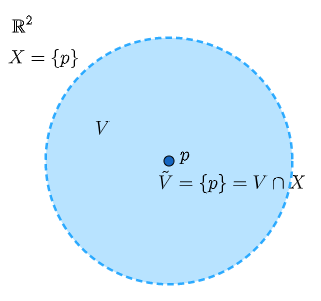
\includegraphics[scale=0.5]{./img/ejemplo-dimension-1.png} &   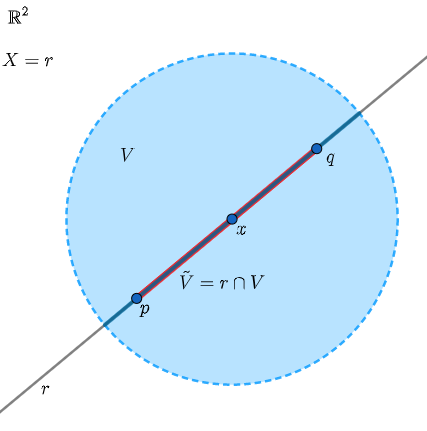
\includegraphics[scale=0.45]{./img/ejemplo-dimension-2.png} \\
(a) Ejemplo con $X=\{p\}$ & (b) Ejemplo con $X=r$ \\[6pt]
\end{tabular}
\caption{Figuras representativas de los ejemplos}
\label{fig:ejemplos}
\end{figure}


\begin{ejemplo}
\label{ej:dimension-1}
(Véase imagen \ref{fig:ejemplos} (a))
En $\R^2$ dotado de la topología usual consideramos un punto $p$ cualquiera y el espacio topológico $X=\{p\}$. Por tanto la topología inducida por la topología usual $\tau$ en $X$ es $\tau_X=\{X,\emptyset\}$. Sea $V$ un abierto de $\R^2$ que contenga a $p$, por tanto $\tilde{V} = V \cap X = \{p\}$ es un abierto en $X$ que contiene a $p$. Podemos encontrar entonces un abierto $U=\{p\}$ de $X$ tal que su frontera $\partial(U)=\emptyset$ y además $p\in U \subseteq V$. Por tanto concluimos que $X$ tiene dimensión 0.
\end{ejemplo}

\begin{ejemplo}
(Véase imagen \ref{fig:ejemplos} (b))
En $\R^2$ dotado de la topología usual, consideramos una recta cualquiera, llamémosla $r$, y el espacio topológico $X=\{r\}$. Sea $x\in X$ y $V$ un abierto de $\R^2$ que contenga a $x$, de forma que $\tilde{V} = r\cap V$ es un abierto de $X$. Podemos entonces tomar un abierto $U$ dentro de $\tilde{V}$ (un segmento abierto de recta), de forma que $x\in U\subseteq \tilde{V}$. Por otro lado, $\partial(U)=\{p,q\}$, y podemos comprobar fácilmente (con ayuda del ejemplo \ref{ej:dimension-1}) que $\dim_T(\partial(U))=0$. Por todo esto podemos concluir que $X=r$ es un espacio topológico de dimensión 1. 
\end{ejemplo}

\subsection{Relación entre los distintos tipos de dimensión fractal}

La dimensión por cajas, aunque útil en la práctica, al comienzo de la sección \ref{subsection:dim-Hausdorff} hemos comprobado que tiene algunos problemas. No obstante, para muchos fractales, y en particular para los que cumplen la \textit{condición de conjunto abierto}\footnote{Wagon, S. (2010). Mathematica in Action. Springer Publishing. p. 124}, resulta más sencillo computacionalmente calcular su dimensión por cajas frente a su dimensión de Hausdorff.

En general, y como se puede comprobar en \cite[Sección 3.1]{alma991007022459704990}, ocurre que la dimensión por cajas acota superiormente a la dimensión de Hausdorff, esto es, dado $A\subset\R^n$:
$$
\dim_H(A)\leq\diminf (A) \leq \dimsup (A),
$$
donde, insistimos, es posible que se dé la igualdad.

Sobre la dimensión topológica, se tiene que si $X$ es un espacio topológico separable\footnote{Recordamos que un espacio topológico es \textit{separable} si contiene un conjunto denso numerable}, entonces
$$
\dim_T(X)\leq\dim_H(X).
$$

Este resultado fue originalmente probado por \textit{Edward Szpilrajn}, véase \cite[Capítulo VII]{Hurewicz-Wallman}.

Por otro lado, si nos restringimos a conjuntos totalmente autosimilares, existe un resultado que relaciona la dimensión de Hausdorff y la dimensión por cajas para conjuntos totalmente autosimilares: el teorema de Moran \cite{Moran}. Este resultado nos asegura que en estos casos la dimensión por cajas y la dimensión de Hausdorff coinciden.

En conclusión, para un conjunto no vacío y acotado $A\subseteq\R^n$, se tiene que:

\begin{equation}
  \label{eq:desigualdades-dimensiones}
  \dim_T(A)\leq\dim_H(A)\leq\dim_B(A)\leq n
\end{equation}

A partir de esta cadena de desigualdades, en la que notamos que la dimensión fractal, entendiendo por esta la dimensión de Hausdorff que es la más general, y que siempre excede o iguala a la dimensión topológica, podemos enunciar nuestra primera definición de fractal, que fue formulada por \textit{Benoit Mandelbrot} en \cite{alma991007242979704990}.

\begin{definicion}[Fractal]
\label{def:fractal}
Un \textbf{fractal} es un subconjunto de $\R^n$ que es autosimilar y cuya dimensión fractal excede a su dimensión topológica.
\end{definicion}